%Đây là template dùng cho đề cương đề tài tốt nghiệp
%Khoa Công nghệ Thông tin
%Trường Đại học Khoa học Tự nhiên, ĐHQG-HCM

%Liên hệ về mẫu LaTEX này: Thầy Bùi Huy Thông (bhthong@fit.hcmus.edu.vn)

\documentclass{article}[14pt]
\usepackage[utf8]{vietnam}
\usepackage{enumerate}
\usepackage{enumitem}
\usepackage{multicol}
\usepackage{listings}
\usepackage[left=2cm,right=2cm,top=2.5cm,bottom=2.5cm]{geometry}
\usepackage{verbatim}
\usepackage{graphicx}
\usepackage{url}
\usepackage{fancyhdr}
\usepackage{fancybox,framed}
\linespread{1.3}
\usepackage{lastpage}
\usepackage{floatrow}
\usepackage{array}
\pagenumbering{arabic}
%\pagestyle{fancy}
\newfloatcommand{capbtabbox}{table}[][\FBwidth]

% \usepackage{tabularx}
\usepackage{blindtext}
\usepackage{titlesec}
\usepackage[nottoc]{tocbibind}
\usepackage{parskip}
\usepackage{longtable}
\usepackage{float}
\usepackage{makecell, cellspace, caption}
\newcolumntype{L}[1]{>{\raggedright\let\newline\\\arraybackslash\hspace{0pt}}m{#1}}
\newcolumntype{C}[1]{>{\centering\let\newline\\\arraybackslash\hspace{0pt}}m{#1}}
\newcolumntype{R}[1]{>{\raggedleft\let\newline\\\arraybackslash\hspace{0pt}}m{#1}}


\titleformat*{\section}{\LARGE\bfseries}
\titleformat*{\subsection}{\Large\bfseries}
\titleformat*{\subsubsection}{\Large\bfseries}
\setlength\parindent{0pt}
\setlength{\parskip}{5pt}

\begin{document}
\begin{figure}[h]
    \begin{floatrow}
        \ffigbox{
\includegraphics[scale = .4]{images/logo.png}}
        {%

        }
        \capbtabbox{
            \begin{tabular}{l}
                \multicolumn{1}{c}{\textbf{\begin{tabular}[c]{@{}c@{}}TRƯỜNG ĐẠI HỌC KHOA HỌC TỰ NHIÊN\\KHOA CÔNG NGHỆ THÔNG TIN\end{tabular}}} \\ \\ \\
            \end{tabular}
        }
        {%

        }
    \end{floatrow}
\end{figure}

\begin{center}

    %Xác định loại đề tài tốt nghiệp tương ứng: Khóa luận, Thực tập, Đồ án
    \textbf{\huge ĐỀ CƯƠNG KHOÁ LUẬN TỐT NGHIỆP} \\
\end{center}

%\vspace{.5cm}

\begin{center}
    %Tên đề tài phải VIẾT HOA

    \textbf{\Large HỆ THỐNG UY TÍN \\ PHỤC VỤ XÁC THỰC HỒ SƠ VÀ ĐÁNH GIÁ KỸ NĂNG}
    \\

    %Tên đề tài bằng tiếng Anh (nếu có)
    \vspace{.5cm}
    \textbf{\Large (Reputation system for résumé verification and skill assessment)}
\end{center}

\vspace{.5cm}

\Large
\section{THÔNG TIN CHUNG}
\begin{itemize}[label = {}]

    \item \textbf{Giảng viên hướng dẫn:}
          %Thể hiện dạng: <Chức danh> <Họ và tên> (<Đơn vị công tác>)
          \begin{itemize}
              PGS.TS. Nguyễn Đình Thúc
          \end{itemize}{}


    \item \textbf{Nhóm sinh viên thực hiện:}

          %Thể hiện dạng: <Họ và tên sinh viên> (MSSV: )
          \begin{enumerate}
              \item Nguyễn Hải Tuyên (MSSV: 21127474)
              \item Trần Minh Đạt (MSSV: 21127570)
          \end{enumerate}

          %Chọn loại thích hợp
    \item \textbf{Loại đề tài:} Ứng dụng

    \item \textbf{Thời gian thực hiện:} Từ 3/2025 đến 8/2025


\end{itemize}

\pagebreak

\section{NỘI DUNG THỰC HIỆN}
 {

  \subsection{Giới thiệu về đề tài}

  Trong quá trình tuyển dụng nguồn nhân lực hiện nay đối với các ngành nghề, đặc biệt là Công nghệ thông tin,
  việc xác thực trình độ học vấn, kỹ năng và kinh nghiệm của một cá nhân vẫn còn gặp nhiều khó khăn.
  Hiện nay, các nhà tuyển dụng và doanh nghiệp thường dựa vào chứng chỉ, bằng cấp hoặc thông tin do ứng viên cung cấp để đánh giá năng lực.
  Tuy nhiên, những thông tin này \textbf{có thể bị làm giả} hoặc không phản ánh chính xác thực lực của ứng viên.

  Bên cạnh đó, nhiều cá nhân có kỹ năng thực tế nhưng lại không có cách nào để chứng minh năng lực của mình ngoài những hồ sơ truyền thống.
  Điều này làm hạn chế cơ hội phát triển và nâng cao giá trị cá nhân trong ngành.
  Vì vậy, cần có một giải pháp minh bạch, khách quan và đáng tin cậy để xác thực trình độ của mỗi cá nhân,
  đồng thời giúp doanh nghiệp dễ dàng đánh giá năng lực của ứng viên một cách chính xác hơn.

  Theo đó, ý tưởng về một \textbf{Hệ thống uy tín phục vụ xác thực hồ sơ và đánh giá kỹ năng} được phát triển dựa trên công nghệ blockchain,
  cung cấp một nền tảng giúp cá nhân có thể chứng minh năng lực của mình một cách minh bạch, công khai và không thể thay đổi.
  Hệ thống cho phép người dùng tham gia các thử thách để kiểm tra và chứng minh kỹ năng, đồng thời áp dụng cơ chế đánh giá phi tập trung để đảm bảo tính khách quan.

  Thay vì chỉ dựa vào văn bằng, chứng chỉ hay lời khai của ứng viên, hệ thống này sẽ ghi nhận kết quả đánh giá được tích lũy lên blockchain và dịch vụ lưu trữ phi tập trung,
  giúp tạo ra một hồ sơ uy tín đáng tin cậy, có thể sử dụng trên nhiều nền tảng khác nhau.
  Cộng đồng chuyên gia và nhà tuyển dụng có thể tham gia vào quá trình đánh giá để đảm bảo chất lượng,
  đồng thời giúp thúc đẩy sự phát triển của một hệ sinh thái xác thực năng lực trong lĩnh vực Công nghệ thông tin.

  \subsection{Mục tiêu đề tài}

  Đề tài nhằm xây dựng một hệ thống uy tín phi tập trung ứng dụng công nghệ blockchain để xây dựng và xác thực kỹ năng và hồ sơ cá nhân, bước đầu giới hạn trong lĩnh vực Công nghệ thông tin.
  Hệ thống sẽ cung cấp một môi trường và phương thức đánh giá minh bạch, khách quan và không thể thay đổi, giúp cá nhân chứng minh năng lực thực tế một cách đáng tin cậy,
  đồng thời hỗ trợ tổ chức và doanh nghiệp trong việc xác thực trình độ ứng viên.

  Hệ thống hướng đến việc \textbf{tạo lập một môi trường đánh giá công bằng}, nơi mà năng lực của cá nhân được thể hiện thông qua kết quả thực tế,
  thay vì chỉ dựa vào chứng chỉ hoặc hồ sơ tự khai. Bên cạnh đó, việc ứng dụng blockchain giúp đảm bảo dữ liệu được bảo mật,
  minh bạch và có thể truy xuất dễ dàng, góp phần nâng cao độ tin cậy và hiệu quả trong quy trình tuyển dụng và đánh giá nhân sự.

  Ngoài việc giải quyết bài toán xác thực hồ sơ, hệ thống còn tạo động lực để cá nhân \textbf{phát triển kỹ năng liên tục}, khi họ có thể tham gia các thử thách
  để cải thiện năng lực và nhận được sự công nhận từ cộng đồng. Với tiềm năng mở rộng, mô hình này có thể được áp dụng cho nhiều lĩnh vực khác,
  đóng góp vào xu hướng phát triển của các giải pháp phi tập trung trong tương lai.

  \subsection{Phạm vi của đề tài}

  Đề tài tập trung nghiên cứu và phát triển một hệ thống uy tín phi tập trung dựa trên blockchain để xác thực kỹ năng và hồ sơ cá nhân trong lĩnh vực Công nghệ thông tin.
  Hệ thống sẽ cung cấp một cơ chế minh bạch, khách quan nhằm đánh giá năng lực cá nhân dựa trên kết quả thực tế thay vì chỉ dựa vào chứng chỉ hoặc hồ sơ tự khai.

  \subsubsection{Đối tượng nghiên cứu}
  \begin{itemize}
      \item \textbf{Công nghệ blockchain} và ứng dụng trong hệ thống uy tín.
      \item \textbf{Smart Contract} để tự động hóa quy trình xác thực, đánh giá, truy vấn và lưu trữ.
      \item \textbf{Dịch vụ lưu trữ phi tập trung} để lưu trữ nội dung dữ liệu lớn như thử thách, giải pháp\dots
      \item \textbf{Cơ chế đánh giá phi tập trung} dựa trên sự tham gia của cộng đồng.
      \item \textbf{Hệ thống quản lý uy tín} giúp cá nhân tích lũy điểm số và nâng cao uy tín.
  \end{itemize}

  \subsubsection{Thực thể liên quan}
  \begin{itemize}
      \item \textbf{Người dùng:} bao gồm học sinh, sinh viên và người đi làm trong lĩnh vực Công nghệ thông tin, cũng như các tổ chức, doanh nghiệp có nhu cầu đánh giá kỹ năng của ứng viên hoặc nhân sự.
      \item \textbf{Smart Contract:} xử lý cơ chế đánh giá, chấm điểm, xác thực, truy vấn và lưu trữ dữ liệu trên blockchain.
      \item \textbf{Decentralized Storage} (DeStor): dịch vụ lưu trữ phi tập trung để lưu trữ dữ liệu lớn không cần thiết lưu on-chain.
  \end{itemize}

  \subsubsection{Tập dữ liệu}
  \begin{itemize}
      \item \textbf{Ngân hàng thử thách}: kho tàng các thử thách được đóng góp bởi các người đóng góp, mỗi thử thách sẽ có tiêu đề, mô tả, loại thử thách, lượng token treo thưởng, v.v.
      \item \textbf{Bộ kết quả kiểm duyệt}: một thử thách sẽ nhận được nhiều điểm số từ nhiều người kiểm duyệt khác nhau trước khi nó được công khai cho người học tham gia.
      \item \textbf{Bộ danh sách giải pháp}: một thử thách sẽ có nhiều giải pháp khác nhau được cung cấp bởi nhiều người học khác nhau.
      \item \textbf{Bộ kết quả đánh giá}: một giải pháp sẽ nhận được nhiều điểm số từ nhiều người đánh giá khác nhau.
      \item \textbf{Danh sách bài tuyển dụng}: các bài tuyển dụng được đăng tải bởi các đội ngũ tuyển dụng, mỗi bài tuyển dụng sẽ có tiêu đề, mô tả công việc, yêu cầu về điểm uy tín, v.v.
      \item \textbf{Bộ thông tin ứng tuyển}: một bài tuyển dụng sẽ được nhiều người dùng khác nhau ứng tuyển.
      \item \textbf{Danh sách các cuộc họp trực tuyến}: những buổi gặp mặt trực tuyến được lên lịch bởi đội ngũ tuyển dụng dành cho một dùng cho một bài tuyển dụng nhất định.
      \item \textbf{Hồ sơ người dùng}:
            \begin{itemize}
                \item Thông tin cá nhân, chẳng hạn như địa chỉ ví, tên, email, ảnh đại diện, v.v.
                \item Chỉ số uy tín của người dùng trên hệ thống
                \item Lịch sử tham gia thử thách
            \end{itemize}
      \item \textbf{Thông tin giao dịch}: phản ánh việc đóng góp, kiểm duyệt và tham gia thử thách, đánh giá giải pháp, đăng bài tuyển dụng và ứng tuyển, và sự biến động về chỉ số uy tín.
  \end{itemize}

  \subsubsection{Giới hạn và ràng buộc của đề tài}
  \begin{itemize}
      \item Chỉ tập trung vào lĩnh vực Công nghệ thông tin, chưa áp dụng cho các ngành khác.
      \item Không đánh giá qua kinh nghiệm làm việc, chỉ dựa trên thử thách kỹ năng trên nền tảng này.
      \item Phạm vi triển khai ban đầu sẽ giới hạn ở quy mô thử nghiệm, trước khi mở rộng áp dụng rộng rãi.
  \end{itemize}

  \subsection{Cách tiếp cận dự kiến}
  %Có thể bổ sung hình ảnh vào để làm rõ phương pháp hoặc cách tiếp cận dự kiến.

  % Giới thiệu một số nghiên cứu (trong hoặc ngoài nước) đã được tiến hành theo hướng nghiên cứu của đề tài, nêu kết quả và nhận xét với các nghiên cứu này. Các trích dẫn từ các tài liệu sử dụng theo định dạng của tổ chức IEEE. Các ví dụ kế tiếp thể hiện trích dẫn tài liệu từ sách (\cite{latexcompanion}), từ bài báo trong tạp chí (\cite{einstein}) hay từ đường dẫn đến website (\cite{knuthwebsite}). \newline
  % Nêu các phương pháp, cách tiếp cận cũng như mô hình dự kiến thực hiện trong đề tài, chỉ rõ sự khác biệt (nếu có) so với các nghiên cứu đã được tiến hành ở trên.

  \subsubsection{Tổng quan về các nghiên cứu liên quan}
  Trong phần này, chúng tôi sẽ trình bày tổng quan những nghiên cứu đã được tiến hành theo hướng nghiên cứu của đề tài hệ thống uy tín (Reputation System), bao gồm những nghiên cứu trong nước và những nghiên cứu ngoài nước.
  \par
  % Nghiên cứu trong nước
  Đối với nghiên cứu trong nước, bài nghiên cứu "Quản Lý Định Danh Phi Tập Trung" \cite{quan-ly-dinh-danh-phi-tap-trung} là xuất phát điểm quan trọng của đề tài. Ý tưởng chính của bài nghiên cứu là việc xây dựng một thống quản lý định danh số nơi người dùng (chủ thể định danh) có toàn quyền kiểm soát đối với thông tin định danh của mình, thay vì phụ thuộc vào các nhà cung cấp dịnh vụ (service provider). Bài nghiên cứu đã đề xuất việc sử dụng công nghệ chuỗi khối (blockchain) để xây dựng hệ thống định danh, bao gồm hai chủ thể chính: người dùng (chủ thể định danh) và nhà cung cấp dịnh vụ (service provider). Dữ liệu định danh của người dùng được lưu trữ cục bộ trên chính thiết bị của người dùng dưới dạng mã hóa và tham chiếu đến dữ liệu được lưu trên chuỗi khối (blockchain). Để quản lý dữ liệu mã hóa, cả chủ thể định danh và nhà cung cấp dịch vụ cần sử dụng giao thức tương tác DataTX. Chủ thể định danh có toàn quyền đối với dữ liệu của mình, có thể quản lý quyền truy cập thông qua giao thức tương tác AccessTx.
  \par
  Bài nghiên cứu cũng đã định nghĩa về uy tín (reputation) như sau: "Uy tín được hình thành và biến đổi qua những thành công hay thất bại thực thể khi thực thi các nhiệm vụ cụ thể" \cite{quan-ly-dinh-danh-phi-tap-trung,a-survey-of-trust-in-internet-applications}. Có thể hiểu rằng, uy tín không phải là thực thể bất biến, mà luôn thay đổi theo thời gian và từng ngữ cảnh cụ thể. Không chỉ dừng lại ở một khái niệm lý thuyết đơn thuần, bài nghiên cứu đã đề xuất một hướng tiếp cận cụ thể để tính toán và số hóa khái niệm trừu tượng này bằng cách dựa vào hành vi (behavior) của các Node trong mạng, bao gồm người dùng (chủ thể định danh) và nhà cung cấp dịch vụ (service provider). Niềm tin của một thực thể (Node) được thiết lập là "giá trị kỳ vọng về hành vi tốt của Node trong tương lai" \cite{quan-ly-dinh-danh-phi-tap-trung}. Kỳ vọng này chính là xác suất \(p\) trong phân phối Bernoulli, được tính bằng cách đếm số hành động của Node để tính xấp xỉ xác suất. \cite{thong-ke-may-tinh,quan-ly-dinh-danh-phi-tap-trung}
  \par
  % Nghiên cứu ngoài nước
  Đối với các nghiên cứu ngoài nước, chúng tôi đã tham khảo từ các bài báo của dự án Rebooting the Web Of Trust (RWOT) \cite{reputation-toolkit, reputation-design, reputation-interpretation}. Các công trình này đã đưa ra một khung khái niệm (conceptual framework) cơ bản cho một hệ thống uy tín, đặc biệt trong việc đánh giá kỹ năng của một cá nhân khi tham gia vào mạng.
  \par
  Bài báo \cite{reputation-toolkit} đã đề xuất một quy trình chung gồm các bước thao tác của các thực thể trong một hệ thống uy tín:
  \begin{itemize}
      \item Mỗi cá nhân tham gia vào mạng bằng một mã định danh phi tập trung (DID - Distributed Identifier).
      \item Chủ thể cần xây dựng uy tín sẽ tạo một tuyên bố (Assertion) và ký bằng khóa bí mật (private key) của mình.
      \item Để tăng tính thuyết phục của tuyên bố (Assertion), chủ thể có thể tạo một bằng chứng (Evidence) và ký bằng khóa bí mật (private key) của mình, sau đó bổ sung tuyên bố ban đầu bằng cách tham chiếu đến bằng chứng vừa tạo.
      \item Các chủ thể khác tạo một bài đánh giá (Evaluation), ký bằng khóa bí mật của mình và tham chiếu đến tuyên bố (Assertion) của chủ thể cần xây dựng uy tín. Một bài đánh giá có thể ủng hộ (support) hoặc thách thức (challenge) tuyên bố gốc, có thể tham chiếu đến các bằng chứng (Evidence) để tăng tính thuyết phục.
      \item Cộng đồng sẽ tham gia bình chọn cho các bài đánh giá. Họ có thể lựa chọn đồng tình hoặc không đồng tình với bài đánh giá.
  \end{itemize}
  Bài báo \cite{reputation-design} đã chỉ ra các yếu tố cốt lõi cần xem xét khi xây dựng một hệ thống uy tín phi tập trung, bao gồm bối cảnh (Context); sự tham gia của cộng đồng (Participation); sự đồng thuận của người dùng (User Consent); tính bảo mật (Confidentiality), khả năng tạo giá trị (Value Generation); hiệu suất hệ thống (Performance); tính bền vững của hệ thống (Sustainability); vòng đời của các tuyên bố (Claim Lifecycle); tính phục hồi sau các cuộc tấn công mạng (Resilience) và khía cạnh pháp lí (Legal).
  \par
  Và bài báo \cite{reputation-interpretation} đã tập trung vào việc tìm kiếm giải pháp để số hóa khái niệm trừu tượng uy tín. Uy tín của một chủ thể phụ thuộc vào rất nhiều yếu tố và ngữ cảnh khác nhau, vì vậy việc biến những dữ liệu thô đầu vào thành dữ liệu đầu ra nhất quán, có thể xử lý được (actionable output) là một phần quan trọng trong một hệ thống uy tín. Cụ thể hơn, bài báo đã đưa ra một quy trình tuần tự, bao gồm việc xác định dữ liệu đầu ra (output), xác định dữ liệu thô đầu vào (raw input), xác định chất lượng đầu vào và biên độ lỗi, chuẩn hóa dữ liệu để đưa về một dạng nhất quán, và cuối cùng là xử lý dữ liệu.
  \par
  Nhìn chung, các nghiên cứu, bài báo mà chúng tôi đã tham khảo từ trong và ngoài nước đã định hình một ý tưởng sơ khai về một hệ thống uy tín phi tập trung. Các nghiên cứu, bài báo đã đề xuất những quy trình xử lý, cách thức tương tác giữa các chủ thể trong hệ thống, kiến trúc hệ thống, cũng như các khía cạnh cần xem xét trong một hệ thống uy tín. Qua đó, đã tạo tiền đề cho bài nghiên cứu này về việc xây dựng và triển khai một hệ thống uy tín trong thực tiễn.

  \subsubsection{Phương pháp và cách tiếp cận dự kiến}
  Từ ý tưởng rút ra từ các nghiên cứu và bài báo đã tiến hành theo hướng đề tài này, chúng tôi đã nghiên cứu và thiết kế kiến trúc sơ bộ của hệ thống như hình \ref{fig:architect}. Hệ thống sẽ bao gồm các chủ thể tương tác sau:
  \begin{itemize}
      \item \textit{Người đóng góp} (Contributor): Là những người dùng tạo các thử thách (Challenge), có trách nhiệm đóng góp ngân hàng thử thách của hệ thống.
      \item \textit{Người kiểm duyệt} (Moderator): Là những người có trách nhiệm kiểm duyệt các thử thách do người đóng góp tạo ra, thực hiện phân loại, đánh giá, và kiểm định chất lượng của thử thách. Để trở thành người kiểm duyệt, người dùng phải thỏa mãn các điều kiện cụ thể được quy định bởi hệ thống.
      \item \textit{Người học} (Talent): Là những người có nhu cầu xây dựng uy tín, có thể tìm kiếm các thử thách, tham gia và đưa ra các giải pháp (Solution) tương ứng.
      \item \textit{Người đánh giá} (Evaluator): Là những người tham gia vào quá trình đánh giá giải pháp mà người dùng đưa ra cho một thử thách.
      \item \textit{Phòng tuyển dụng của các công ty}: Là đội ngũ tuyển dụng của các công ty có nhu cầu tuyển dụng những ứng viên phù hợp.
  \end{itemize}

  \begin{figure} [h!]
      \centering
      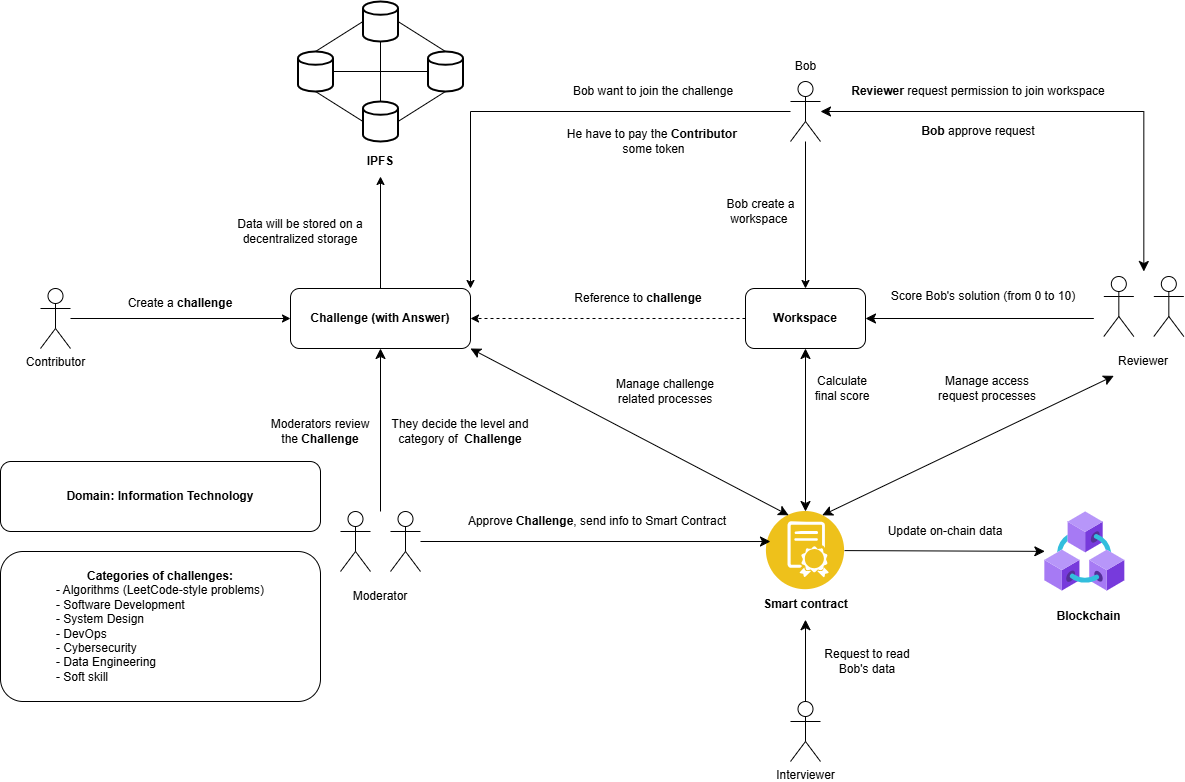
\includegraphics[width=0.97\textwidth]{images/prototype-v1.1.png}
      \caption{Sơ đồ hoạt động hệ thống dự kiến}
      \label{fig:architect}
  \end{figure}

  \begin{enumerate}[label=\textbf{\alph*.}]
      \item \textbf{Các thành phần công nghệ chính:}
            \begin{itemize}
                \item Blockchain: Sổ cái phi tập trung, có vai trò lưu trữ dữ liệu quan trọng trên chuỗi (on-chain) như thông tin người dùng, danh sách thử thách, danh sách giải pháp, chỉ số uy tín, quyền truy cập vào dữ liệu của người dùng, \dots Dữ liệu có thể chứa các tham chiếu (CID) của các dữ liệu lưu ngoài chuỗi (off-chain).
                \item Smart Contract: Hợp đồng thông minh tương tác với blockchain để quản lý dữ liệu on-chain, đồng thời thực thi các tiến trình quan trọng như: tính toán chỉ số uy tín, cập nhật kết quả lưu trên chuỗi, thực hiện các biện pháp phạt theo quy ước.
                \item DeStor: Giải pháp lưu trữ phi tập trung dùng để lưu trữ dữ liệu người dùng, nội dung của các \textit{thử thách} (Challenge), các \textit{giải pháp} (Solution) của nó, và các dữ liệu lớn cần lưu trữ ngoài chuỗi (off-chain).
            \end{itemize}

      \item \textbf{Kịch bản tương tác giữa các chủ thể:}
            \begin{itemize}
                \item \textbf{Tạo thử thách}
                      \begin{itemize}
                          \item Người đóng góp tạo và đăng tải các thử thách lên hệ thống, mỗi thử thách phải thuộc về một loại thử thách nhất định (ví dụ: Quản trị cơ sở dữ liệu, An ninh mạng, Phát triển phần mềm, v.v. ).
                          \item Hệ thống lưu nội dung của thử thách ở DeStor. Smart Contract cập nhật danh sách các thử thách trên chuỗi chứa các CID tham chiếu đến nội dung của thử thách ở DeStor.
                          \item Các thử thách vừa tạo ở trạng thái \textit{chờ kiểm duyệt}, cần phải thông qua ý kiến của những người kiểm duyệt.
                          \item Sau giai đoạn kiểm duyệt, nếu thử thách đạt được mức độ phù hợp và được hội đồng tán thành sẽ chuyển sang trạng thái \textit{được chấp nhận}. Những người học cần rèn luyện và chứng minh kỹ năng có thể tham gia vào thử thách.
                      \end{itemize}

                \item \textbf{Kiểm duyệt thử thách}
                      \begin{itemize}
                          \item Những người kiểm duyệt đọc nội dung của thử thách, kiểm tra chất lượng và mức độ phù hợp của thử thách. Sau đó, những người kiểm duyệt tiến hành đề xuất về các thông tin như: độ khó, mức độ phù hợp \dots
                          \item Smart Contract tổng hợp đánh giá và đề xuất của những kiểm duyệt viên, dựa trên một công thức tính đã quy định sẵn để tổng hợp ra kết quả cuối cùng.
                          \item Smart Contract cập nhật thông tin liên quan của thử thách đã lưu trên chuỗi.
                      \end{itemize}

                \item \textbf{Tham gia thử thách và đánh giá}
                      \begin{itemize}
                          \item Người học trả một khoản \textit{phí tham gia} nhất định cho người đóng góp để tham gia thử thách.
                          \item Hệ thống tự động tạo một không gian làm việc nơi người học có thể tạo giải pháp của mình.
                          \item Người học thiết lập một phiên đánh giá với số lượng tối đa người đánh giá cố định có thể tham gia chấm điểm. Người đánh giá có thể đánh giá bằng cách tham gia vào phiên.
                          \item Sau khi hoàn thành đánh giá, mỗi người đánh giá sẽ nộp kết quả đánh giá.
                          \item Smart Contract thu thập tất cả kết quả đánh giá từ người đánh giá, áp dụng thuật toán tính điểm để xác định số điểm cuối cùng.
                          \item Những người đánh giá có điểm số gần với kết quả chính xác nhất sẽ nhận thêm điểm uy tín cho bản thân. Người đánh giá có điểm số lệch xa với kết quả nhất (hoặc biên độ lệch vượt quá giới hạn đã quy định sẵn) sẽ bị trừ đi điểm uy tín.
                          \item Smart Contract sau đó cập nhật kết quả lên blockchain để đảm bảo tính minh bạch và không thể chỉnh sửa.
                          \item Điểm số của giải pháp sẽ làm thay đổi chỉ số uy tín của người giải trong một loại thử thách cụ thể.
                      \end{itemize}

                \item \textbf{Đăng bài tuyển dụng và ứng tuyển}
                      \begin{itemize}
                          \item Đội ngũ tuyển dụng của các công ty tạo và đăng tải các bài tuyển dụng kèm theo yêu cầu về chỉ số uy tín của ứng viên.
                          \item Ứng viên tiến hành ứng tuyển vào các bài tuyển dụng.
                          \item Nhà tuyển dụng lúc này có thể xem được chỉ số uy tín của ứng viên và có thể truy cập lịch sử tham gia thử thách.
                          \item Smart Contract cập nhật dữ liệu quyền truy cập lưu trên chuỗi (nếu có).
                          \item Nhà tuyển dụng có thể lên lịch các cuộc họp trực tuyến để phỏng vấn các ứng viên tiềm năng.
                          \item Đội ngũ tuyển dụng xem xét và quyết định tuyển dụng đối với người dùng. Nếu có, phía công ty cần trả một khoản \textit{phí tuyển dụng} cho hệ thống.
                      \end{itemize}
            \end{itemize}
  \end{enumerate}

  \subsubsection{Sự khác biệt so với các nghiên cứu trước}
  Bài nghiên cứu về hệ thống uy tín mà chúng tôi đang thực hiện thuộc hướng ứng dụng, với mục tiêu xây dựng và triển khai một hệ thống hoàn chỉnh dựa trên cơ sở lý thuyết của các bài nghiên cứu trong và ngoài nước đã được đề cập ở phần trên. Chính vì vậy, bài nghiên cứu này mang tính chất kế thừa, mang định hướng hiện thực hóa các ý tưởng được đề xuất từ các bài nghiên cứu mà chúng tôi đã tham khảo.

  \subsection{Kết quả dự kiến của đề tài}
  Theo dự kiến, kết quả đầu ra của đề tài sẽ là một hệ thống minh họa hoàn chỉnh đảm bảo các yêu cầu:
  \begin{itemize}
      \item Có giao diện tương tác người dùng hoàn chỉnh, đảm bảo thực hiện đầy đủ các chức năng theo yêu cầu.
      \item Thành phần backend của hệ thống bao gồm các Smart Contract được kiểm thử chính xác và triển khai thành công.
      \item Toàn bộ hệ thống có thể chạy được ở máy cục bộ với mục đích minh họa và có thể được triển khai trên một mạng thử nghiệm (testnet) của một blockchain.
  \end{itemize}

  \subsection{Kế hoạch thực hiện}
  Sau đây là bảng kế hoạch dự kiến cho tới hết tháng 6/2025.
  % Phần này mô tả về kế hoạch thực hiện (với các mốc thời gian tương ứng) cùng với việc phân chia công việc cho các thành viên tham gia đề tài. \textit{(Nên thể hiện dưới dạng bảng biểu)}

  \begin{longtable}{| C{4cm} | L{7cm} | L{5cm} |}
      \hline
      %   \rowcolor{Gainsboro!60}
      \makecell{Mốc thời gian} & \makecell{Công việc}                                                                                                                                                                                                                                                                                                                                                                                                                                                                                                                                                                                              & \makecell{Phân công} \\
      \hline
      \endfirsthead
      01/02/2025
                               & Tìm hiểu các công nghệ lập trình ứng dụng phân tán (dApp) như ngôn ngữ lập trình Solidity; khung lập trình Hardhat; các công nghệ chuỗi khối tiềm năng có mức chi phí hợp lí; thư viện hỗ trợ tương tác với chuỗi khối như wagmi, viem, v.v; dịch vụ ví điện tử hỗ trợ tích hợp với dApp như Metamask, CoinBase, v.v; dịch vụ lưu trữ phi tập trung IPFS, Irys, Arweave.
                               & Nguyễn Hải Tuyên, Trần Minh Đạt                                                                                                                                                                                                                                                                                                                                                                                                                                                                                                                                                                                                          \\
      \hline
      01/03/2025
                               & Vẽ kiến trúc hệ thống sơ bộ, mô tả các thành phần cần thiết trong hệ thống, các luồng hoạt động chính của hệ thống cũng như các thành phần công nghệ cần thiết.
                               & Trần Minh Đạt                                                                                                                                                                                                                                                                                                                                                                                                                                                                                                                                                                                                                            \\
      \hline
      08/03/2025
                               & Xây dựng kịch bản tương tác giữa các chủ thể trong hệ thống.
                               & Nguyễn Hải Tuyên                                                                                                                                                                                                                                                                                                                                                                                                                                                                                                                                                                                                                         \\
      \hline
      18/03/2025
                               & Khởi tạo dự án, cài đặt các thư viện, khung lập trình cần thiết.
                               & Trần Minh Đạt                                                                                                                                                                                                                                                                                                                                                                                                                                                                                                                                                                                                                            \\
      \hline
      27/03/2025
                               & Hoàn thiện tính năng đăng nhập, người dùng có thể sử dụng ví điện tử cài đặt sẵn trên trình duyệt để đăng nhập vào hệ thống.
                               & Nguyễn Hải Tuyên                                                                                                                                                                                                                                                                                                                                                                                                                                                                                                                                                                                                                         \\
      \hline
      01/04/2025
                               & Lập trình quản lý thông tin người dùng trong hệ thống, một người dùng cần đảm các thông tin như tên, email, mô tả, v.v. Cần đảm bảo tên người dùng là duy nhất trong hệ thống. Nghiên cứu xây dựng một hợp đồng thông minh quản lý thông tin của người dùng. Xây dựng kiểu dữ liệu User với các trường thông tin cần thiết. Đồng thời, nghiên cứu xây dựng các phương thức cần thiết cho việc truy vấn, cập nhật và xóa dữ liệu. Tích hợp sử dụng dịch vụ lưu trữ phi tập trung như IPFS, Irys, Arweave, v.v đối với các dữ liệu lớn. Bên cạnh đó, sử dụng NextJS để xây dựng giao diện tương tác với người dùng.
                               & Nguyễn Hải Tuyên                                                                                                                                                                                                                                                                                                                                                                                                                                                                                                                                                                                                                         \\
      \hline
      08/04/2025
                               & Hoàn thiện các chức năng của người đóng góp (Contributor) cho phép tạo, chỉnh sửa hoặc xóa các thử thách. Nghiên cứu xây dựng một hợp đồng thông minh quản lý các thử thách trong hệ thống. Xây dựng một kiểu dữ liệu phù hợp cho thử thách và triển khai các phương thức cần thiết. Bổ sung các trường thông tin của người dùng về các thử thách mà họ đã tạo.
                               & Trần Minh Đạt                                                                                                                                                                                                                                                                                                                                                                                                                                                                                                                                                                                                                            \\
      \hline
      15/04/2025
                               & Hoàn thiện các chức năng của kiểm duyệt (Moderator) cho phép đọc dữ liệu và đánh giá. Xác định trường thông tin cần thiết mà người kiểm duyệt cần phải hoàn thiện trước khi nộp biểu quyết. Nghiên cứu và triển khai cơ chế tổng hợp ý kiến của tất cả những người kiểm duyệt. Xây dựng một công thức tính hiệu quả, xác định các trọng số phù hợp như chỉ số uy tín, v.v
                               & Nguyễn Hải Tuyên                                                                                                                                                                                                                                                                                                                                                                                                                                                                                                                                                                                                                         \\
      \hline
      30/04/2025
                               & Hoàn thiện chức năng của người dùng chung cần xây dựng uy tín, cho phép họ tham gia vào các thử thách. Triển khai một không gian riêng của người dùng cho phép người dùng trình bày giải pháp của mình. Bổ sung giao diện tương tác phù hợp về phía frontend.
                               & Trần Minh Đạt                                                                                                                                                                                                                                                                                                                                                                                                                                                                                                                                                                                                                            \\
      \hline
      10/05/2025
                               & Nghiên cứu xây dựng một hợp đồng thông minh triển khai một đồng tiền chung cho hệ thống, token sử dụng phải đảm bảo tuân theo các tiêu chuẩn của ERC20 \cite{ERC20}.
                               & Nguyễn Hải Tuyên                                                                                                                                                                                                                                                                                                                                                                                                                                                                                                                                                                                                                         \\
      \hline
      20/05/2025
                               & Hoàn thiện các chức năng của người đánh giá (Evaluator), cho phép họ xem chi tiết giải pháp khi tham gia vào không gian làm việc của người tạo ra giải pháp. Nghiên cứu xây dựng công thức tính số điểm cuối cùng tổng hợp từ các đánh giá của Evaluator, công thức phải tính đến các trọng số quan trọng như chỉ số uy tín của từng Evaluator. Nghiên cứu triển khai cơ chế đặt cược, thưởng và phạt sau khi tổng hợp được kết quả cuối cùng.
                               & Trần Minh Đạt                                                                                                                                                                                                                                                                                                                                                                                                                                                                                                                                                                                                                            \\
      \hline
      01/06/2025
                               & Hoàn thiện chức năng của các phòng tuyển dụng của các công ty, cho phép họ tìm kiếm hồ sơ của người dùng. Xác định những thông tin nào được công khai theo mặc định, những thông tin nào cần phải có sự đồng ý của người dùng mới có thể truy cập. Nghiên cứu cơ chế trả phí khi các phòng tuyển dụng xác nhận tuyển ứng cử viên.
                               & Nguyễn Hải Tuyên                                                                                                                                                                                                                                                                                                                                                                                                                                                                                                                                                                                                                         \\
      \hline
      20/06/2025
                               & Viết mã nguồn kiểm thử hoàn chỉnh, thực hiện kiểm thử tất cả các tính năng của hệ thống, đảm bảo hệ thống hoạt động ổn định.
                               & Trần Minh Đạt                                                                                                                                                                                                                                                                                                                                                                                                                                                                                                                                                                                                                            \\
      \hline
      30/06/2025
                               & Xử lý các lỗi hệ thống phát hiện được thông qua quá trình kiểm thử, đảm bảo hệ thống hoạt động chính xác.
                               & Nguyễn Hải Tuyên, Trần Minh Đạt                                                                                                                                                                                                                                                                                                                                                                                                                                                                                                                                                                                                          \\
      \hline
  \end{longtable}
 }

\pagebreak
%TÀI LIỆU TRÍCH DẪN
%Đây là ví dụ
\bibliographystyle{ieeetr}
\bibliography{reference}

\begin{center}
    \begin{tabular}{ p{7cm} p{7cm} }
        \textbf{
            \begin{tabular}[c]{@{}c@{}}                  \\
                \normalsize XÁC NHẬN CỦA GVHD \\
                \textit{\normalsize(Ký và ghi rõ họ tên)}
            \end{tabular}
        }
         & \textbf{
            \begin{tabular}[c]{@{}c@{}}
                \textit{\normalsize Tp. Hồ Chí Minh, ngày... tháng... năm...} \\
                \normalsize NHÓM SINH VIÊN THỰC HIỆN                          \\
                \textit{\normalsize(Ký và ghi rõ họ tên)}\end{tabular}
        }
    \end{tabular}
\end{center}

\end{document}